% !TeX spellcheck = en_US

\chapter{Evaluation of the \Acs{tga-ms} Setup}
\label{ap:tga-ms-method}

\begin{figure}
	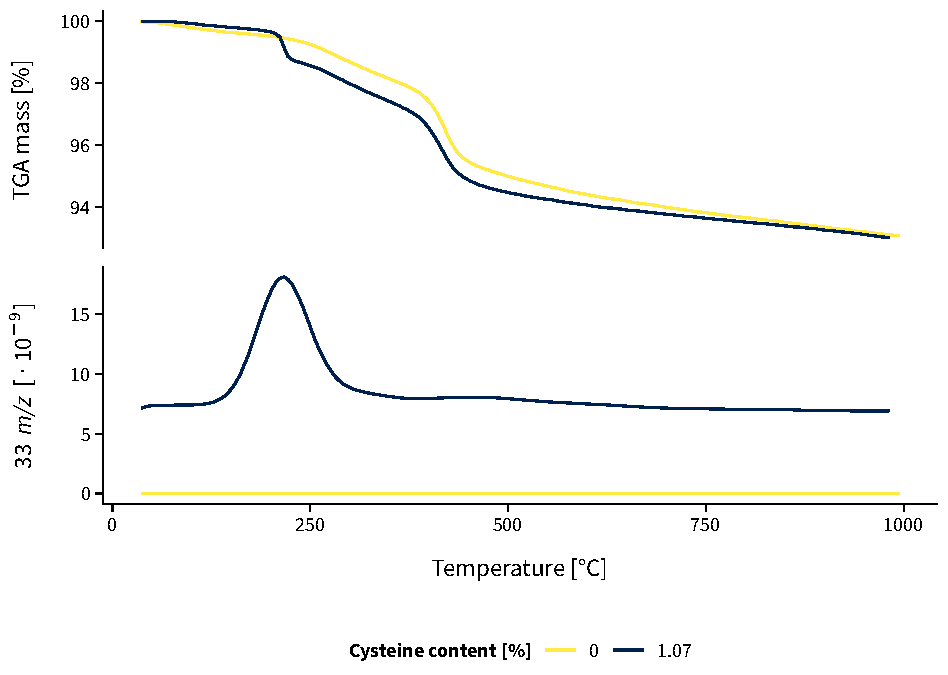
\includegraphics[width=\textwidth]{figures/cysteine-comparison}
	\caption[Exemplary \ac{tga} curves and \SI{33}{\mz} signals of \ac{pet} in soil with and without \textsc{dl}-cysteine as internal standard.]{Exemplary \ac{tga} curves and \SI{33}{\mz} signals of \ac{pet} in soil with and without addition of \textsc{dl}-cysteine (\SI{10.7}{\milli\gram\per\gram}) as internal standard.}
	\label{fig:cysteine-comparison}
\end{figure}

\begin{figure}
	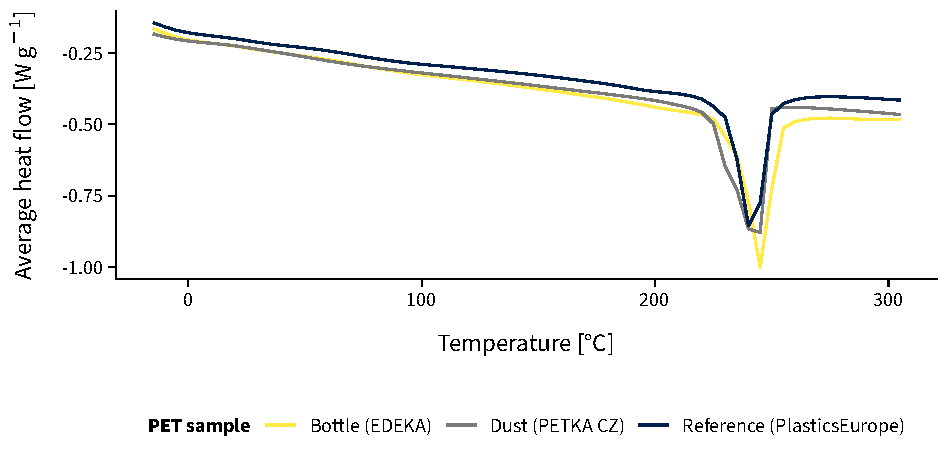
\includegraphics[width=\textwidth]{figures/dsc}
	\caption[Comparison of characteristic melting points of bulk \ac{pet} from a water bottle, ground \ac{pet} recyclate, and \iac{pet} reference.]{Comparison of characteristic melting points (averages from triplicates) of bulk \ac{pet} from a water bottle, ground \ac{pet} recyclate, and \iac{pet} reference.}
	\label{fig:dsc}
\end{figure}

\begin{figure}
	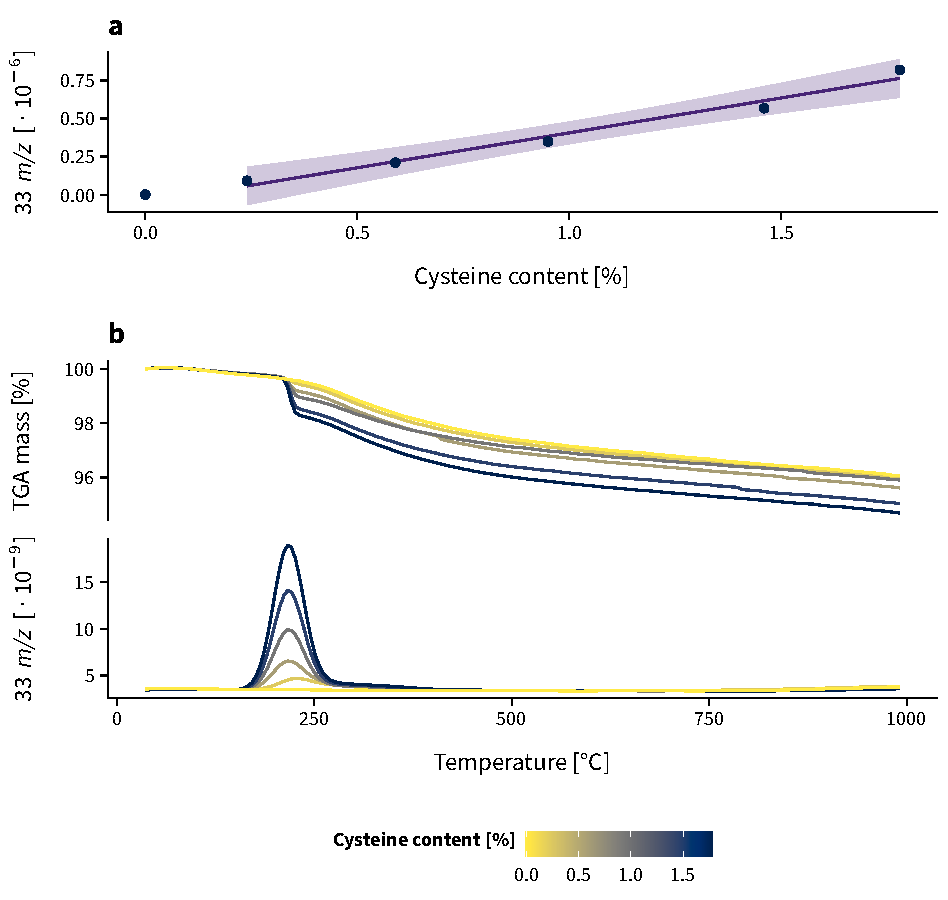
\includegraphics[width=\textwidth]{figures/cysteine-tests}
	\caption[Linear response of \ch{SH-} evolving from \textsc{dl}-cysteine pyrolysis in soil with corresponding \acs{tga} curves.]{(a) Linear response of \ch{SH-} (\SI{33}{\mz}) evolving from \textsc{dl}-cysteine pyrolysis in soil (adj. $R^2$ = \num{0.969}, \acs{rse} = \SI{8.96}{\percent}) with corresponding (b) \acs{tga} curves.}
	\label{fig:cysteine-tests}
\end{figure}

\begin{figure*}
	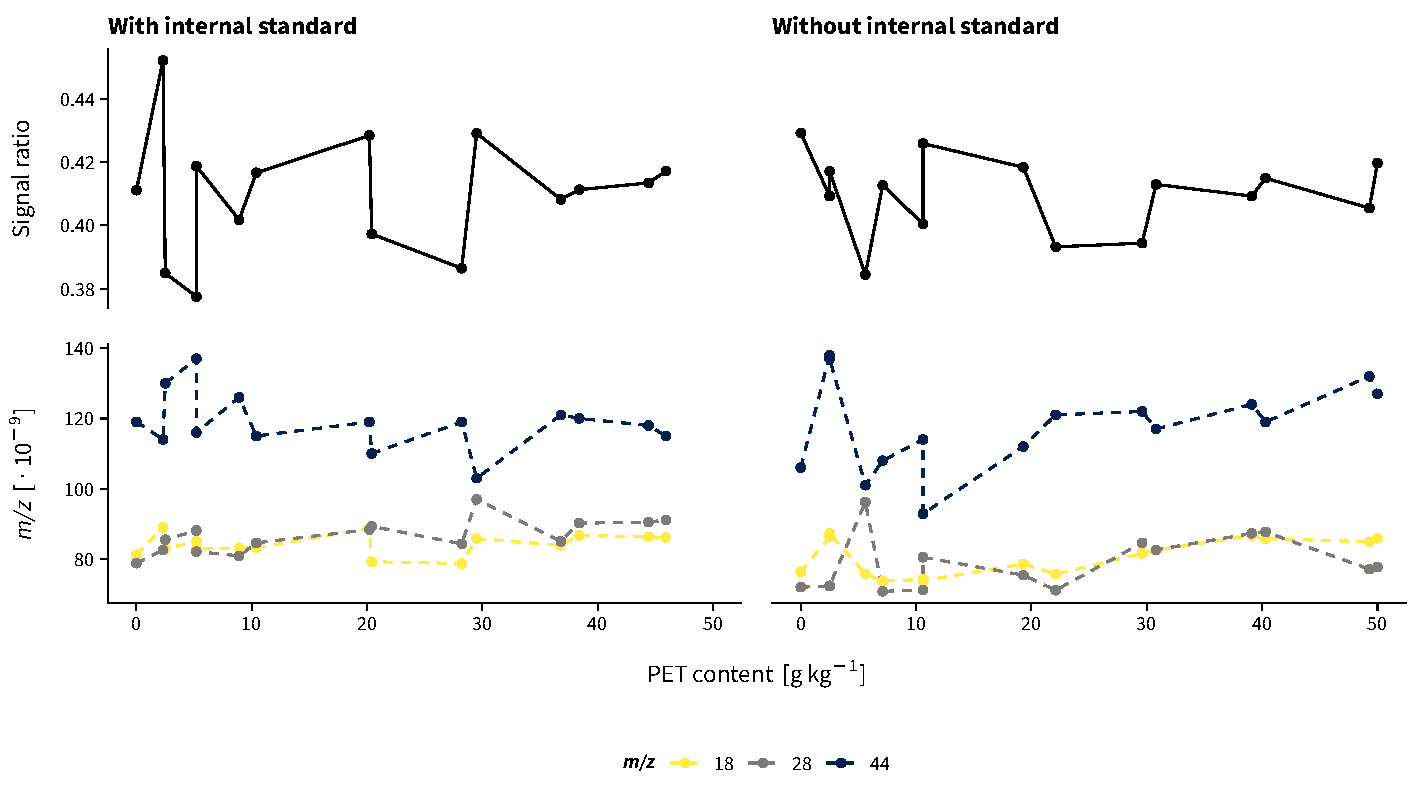
\includegraphics[width=\textwidth]{figures/control-measurements}
	\caption[Integrals of \ch{H2O}, \ch{CO}, and \ch{CO2} from control calcium oxalate hydrate pyrolyses after analyzing \ac{pet}-spiked soil.]{Integrals of \ch{H2O} (\SI{18}{\mz}), \ch{CO} (\SI{28}{\mz}), and \ch{CO2} (\SI{44}{\mz}) from control calcium oxalate hydrate pyrolyses after analyzing \acs{pet}-spiked soil; signal ratio = \SI{18}{\mz} / (\SI{28}{\mz} + \SI{44}{\mz}).}
	\label{fig:control-measurements}
\end{figure*}

\begin{figure}
	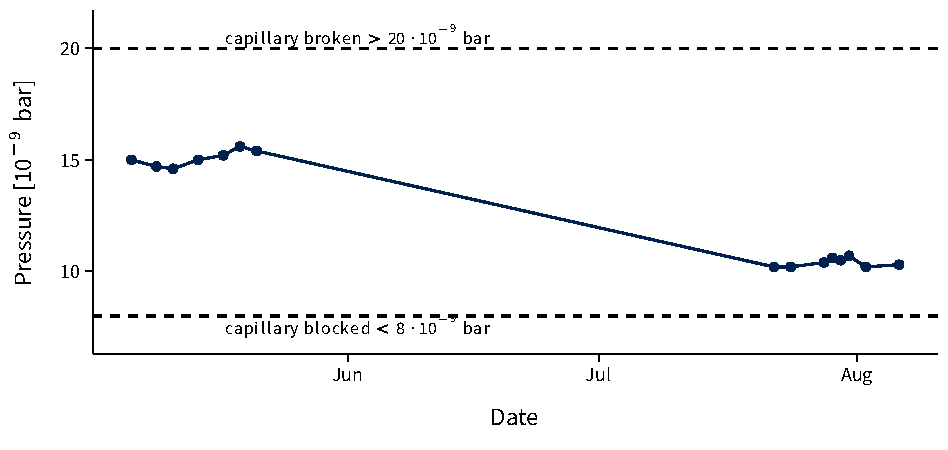
\includegraphics[width=\textwidth]{figures/tga-capillary-pressure}
	\caption{Pressure measurements in the \ac{tga} capillary during analyses.}
	\label{fig:tga-capillary-pressure}
\end{figure}
